%-------------------------------------------------------------------------------
\section{Introduction}
%-------------------------------------------------------------------------------

%-------------------------------------------------------------------------------
\section{Results}
%-------------------------------------------------------------------------------

\subsection{Coherence}

Spectral coherence is the Fourier analogue of linear correlation.
We computed the coherence between the \SIrange{31.3}{97.8}{Hz} range for pairs of depths.
Coherence between channels was computed using the Welch method using \SI{256}{\milli\second} windows with \SI{50}{\percent} overlap.


\begin{figure}[htb]
    \centering
    \subfloat[][\label{fig:lam_coher_lfp}]{
        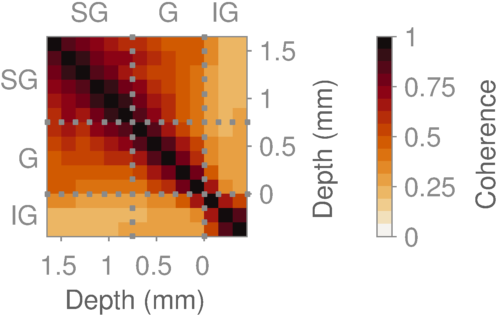
\includegraphics[width=0.47\linewidth]{coherence-avg_paper_Cln.png}
}
    ~~
    \subfloat[][\label{fig:lam_coher_csd}]{
        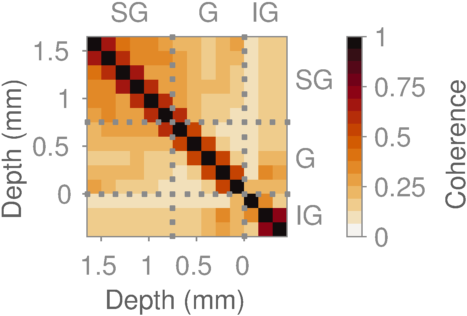
\includegraphics[width=0.47\linewidth]{coherence-avg_paper_Csd.png}
}
    \caption{Coherence \SIrange{31.3}{97.8}{Hz}
\protect\subref{fig:lam_coher_lfp}:~\ac{LFP}.
\protect\subref{fig:lam_coher_csd}:~\ac{CSD}.
}
\label{fig:lam_coher}
\end{figure}

The results show the same compartmentalisation as we observed for the information redundancy in the high frequency range, namely that \ac{G} and \ac{SG} are more correlated in the higher frequency ranges than they are with \ac{IG}.

The results for the coherence of the \ac{LFP} (Fig.~\ref{fig:lam_coher_lfp}) show more coherence than the \ac{CSD} (Fig.~\ref{fig:lam_coher_csd}).
This is to be expected since the \ac{CSD} is a better representation of the current sources within the cortex, whose broad extent induces voltage differences (and hence \ac{LFP}) across a larger amount of cortex.

Our results are in agreement with the observations of \citet[Figure 5B]{Maier2010}.


%-------------------------------------------------------------------------------
\section{Discussion}
%-------------------------------------------------------------------------------
